\chapter{REDES NEURAIS ARTIFICIAIS EM POUCAS PALAVRAS}
\label{cap:redesneuraisempoucaspalavras}

Os principais conceitos de redes neurais e um pouco do contexto histórico serão explanados nesta seção. Primeiramente, o modelo mais simples de RNA que é o Perceptron será apresentado assim como seu sucessor MLP. O Perceptron é usado até hoje em redes mais complexas e por isso é importante elucidar os principais marcos históricos de sua evolução, assim como descrever seus principais componentes e como estes influenciam no aprendizado das RNA mais modernas. Tais conceitos serão empregados na modelagem da RNA que será usada para predizer as propriedades eletrônicas de nanofitas de grafeno.

\section{Perceptron}
\label{sec:perceptron}
O Perceptron é a forma mais simples de uma RNA que pode ser usada para classificação de padrões ditos linearmente separáveis. Ou seja, um Perceptron é capaz de, após treinado, criar um limite de decisão (hiperplano) que, por exemplo, distingue plantas de acordo com os comprimentos e larguras de suas sépalas. 
A tabela \ref{tab:tabela com registros de plantas} contém registros de plantas que são então plotados no gráfico \ref{fig:classes_separadas}. Cada ponto representa uma planta e a cor do ponto depende do tipo da planta sendo azul para o tipo 1 e salmão para o tipo 2.

\begin{table}[!htb]
\centering
\caption{Exemplo de cadastro de tipos de plantas para distinção de classe/tipo de acordo com as dimensões das suas sépalas}
\label{tab:tabela com registros de plantas}
\begin{adjustbox}{max width=\textwidth}
\begin{tabular}{rcSS} 
\toprule
\textbf{Identificação} & \textbf{Planta} & \textbf{Largura} & \textbf{Comprimento} \\
\midrule
1                      & Tipo 1          & 5                & 15                   \\
2                      & Tipo 2          & 10               & 6                    \\
3                      & Tipo 1          & 6                & 17                   \\
4                      & Tipo 2          & 11               & 7                    \\
5                      & Tipo 2          & 12               & 8                    \\
6                      & Tipo 1          & 8                & 12                \\
\bottomrule
\end{tabular}
\end{adjustbox}
\end{table}

Como ilustração, o gráfico abaixo apresenta uma linha, representada pela equação $w_1 * comprimento + w_2 * largura + b = 0 $, que separa os dois tipos de plantas de acordo com as dimensões de largura e comprimento de suas sépalas. Neste caso, um ponto ($x_1, x_2$) que está acima da linha é classificado como planta do tipo 2, e um ponto ($x_1, x_2$) que está abaixo da linha é classificado como planta do tipo 1. Os pesos sinápticos estão representados por $w_1$ e $w_3$. Já o bias $b$ indica onde a linha (hiperplano) corta o eixo vertical.

\begin{figure}[H]
  \centering
  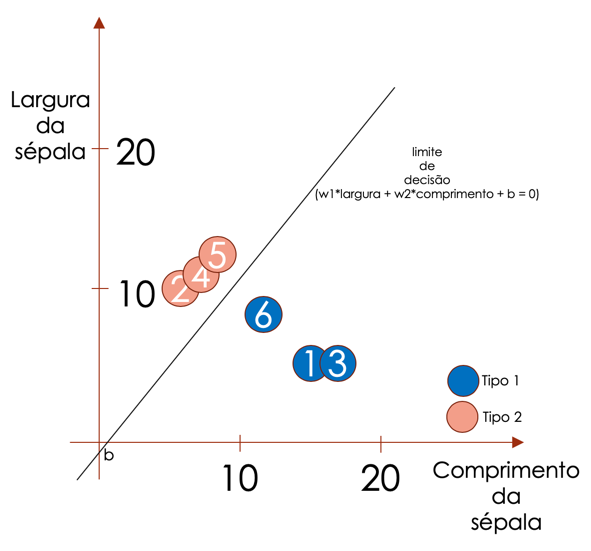
\includegraphics[width=300pt]{figuras/classes_linearmente_separaveis.png}
  \caption{Classes linearmente separáveis}
  \label{fig:classes_separadas}
\end{figure}

Embora apenas nos últimos anos a sociedade tenha absorvido o conceito de aprendizado de máquina, é importante ressaltar que seus princípios foram originados entre os anos de 1943 e 1958, nos quais vários pesquisadores ganharam destaque por contribuições pioneiras como:
\begin{itemize}
    \itemsep-1em
    \item Warren McCulloch e Walter Pitts
    (\citeyear{mcculloch1943logical}) por introduzirem a ideia de redes neurais como máquinas de computação.
    \item Donald Hebb (\citeyear{hebb1949organization}) que postulou a primeira regra de aprendizado auto-organizável.
    \item Frank Rosenblatt (\citeyear{rosenblatt1958two}) que criou um dispositivo eletrônico, de acordo com os princípios biológicos, capaz de aprender de forma supervisionada.
\end{itemize}

O perceptron simples, cria um hiperplano definido pela equação abaixo que separa duas regiões num espaço que abrange $m$ dimensões:
\begin{equation*}
    \sum_{i=1}^{m} w_i * x_i + b = 0
\end{equation*}

Conforme apresentado na figura \ref{fig:perceptron}, os pesos sinápticos do Preceptron são dados por $w_1, w_2, w_3...$. De forma correspondente, as entradas aplicadas ao perceptron são denotadas por $x_1, x_2, x_3...$

\begin{figure}[H]
  \centering
  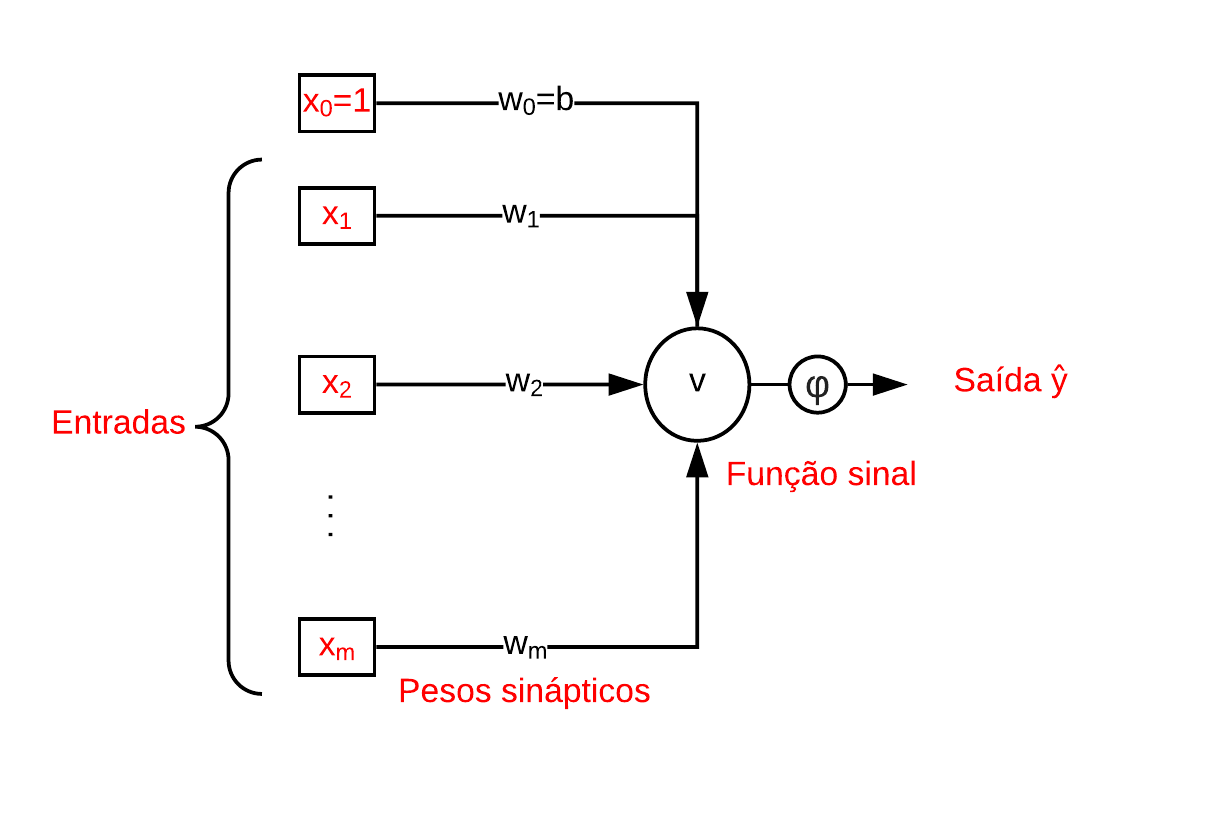
\includegraphics[width=300pt]{figuras/Perceptron.png}
  \caption{Perceptron}
  \label{fig:perceptron}
\end{figure}

Já a função sinal $\phi$ (função de ativação) classifica como 1 (classe 1) se o resultado da combinação linear das entradas pelos seus pesos ($v$) for positivo. Caso contrário, o limitador classifica como -1 (classe 2).

Assumindo que $x$ é o vetor com dimensões $m+1$ por $1$, sendo que o primeiro elemento tem o valor fixo de $+1$ e assumindo que $w$ é vetor de pesos com dimensões $m+1$ por $1$, sendo que o primeiro elemento é igual ao bias $b$, temos que cada computação/iteração $n$ aplica o seguinte ajuste ao vetor de pesos:

\begin{equation*}
\label{eqn:ajustePesoNeuronio}
    w_{n + 1}=w_n + \eta * [d_n - \hat{y}_n] * x_n
\end{equation*}

A maioria algoritmos de aprendizado de máquina tem hiperparâmetros que são variáveis cujos valores são determinados antes do início do treinamento. No caso do Perceptron, o hiperparâmetro taxa de aprendizado $\eta$ indica a intensidade do ajuste aplicado ao vetor de peso na iteração $n$. A convergência da rede neural na separação das classes é garantida independente do valor de $\eta$, mas uma alta taxa de aprendizado resultará num aprendizado mais rápido. É necessário porém, que $0<\eta<=1$ sendo que, de acordo com Lippmann (\citeyear{lippmann1987}), os seguintes conflitos devem ser considerados para a escolha do valor de $\eta$:

\begin{itemize}
    \item Considerar as entradas passadas com mais relevância para prover pesos estáveis, o qual requer um valor pequeno de $\eta$
    \item Rápida apdaptação com respeito às mudanças reais nas distribuições do processo responsável pela geração do vetor de entrada $x$, o qual requer um valor alto para $\eta$ 
\end{itemize}

O modelo Perceptron foi criticado por Minsky e Selfridge (\citeyear{minsky1961steps}) que apontaram que o Perceptron definido por Rosenblatt, mesmo com múltiplas camadas, não poderia nem mesmo generalizar a noção de paridade binária, quanto mais fazer abstrações gerais.
Essa afirmação colocou em cheque o que acreditava-se ser possível com redes neurais até meados de 1980.

No entanto, a conjuctura feita por Minsky e Papert (\citeyear{minsky1969perceptron}) pareceu irrelevante uma vez que modelos mais avançados de redes neurais surgiram. Dentre eles: perceptrons de múltiplas camadas (MLP) com algoritmo de retro-propagação, redes função de base radial (RBF) e máquina de suporte de vetores (SVM). Na seção \ref{sec:redeneuralmlp} a MLP será explicada com mais detalhes.

\section{Rede Neural Artificial Perceptron Múltiplas Camadas}
\label{sec:redeneuralmlp}
Frank Rosenblatt propôs em 1958 o modelo Perceptron que era composto de uma estrutura de rede de neurônios e uma regra de aprendizado. Esse modelo possuía apenas uma camada e tinha como saída um valor
binário. Entretanto, por possuir uma única camada, este modelo podia ser aplicado apenas a problemas linearmente separáveis.
Essa limitação foi resolvida com a criação e aplicação do algoritmo back-propagation (\citeyear{rumelhart1986parallel}) nas redes de múltiplas camadas ou Multi Layer Perceptron (MLP). 

\begin{figure}[H]
    \centering
  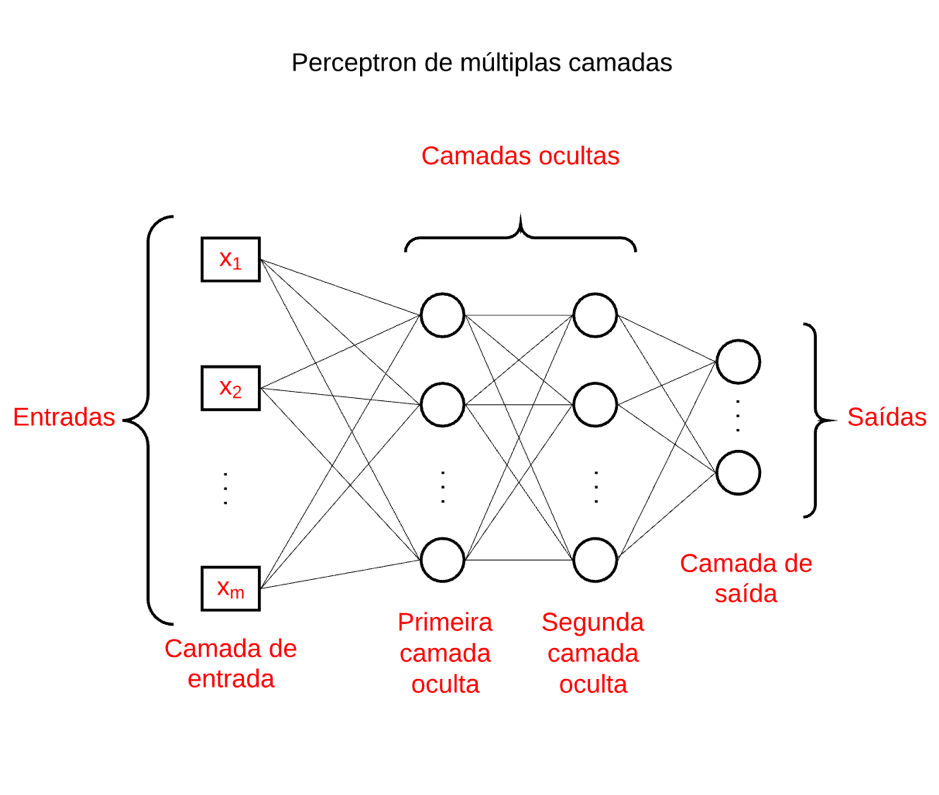
\includegraphics[width=350pt]{figuras/MLP.png}
  \caption{MLP}
  \label{fig:MLP}
\end{figure}

Acima está ilustrada uma arquitetura de rede neural na qual podem ser identificadas a camada de entrada, as camadas ocultas e a camada de saída. Tanto a camada de entrada quanto a camada de saída pode ser uni ou multivalorada. Essa figura representa o primeiro modelo de redes de múltiplas camadas capaz de resolver problemas não linearmente separáveis.

A MLP é uma rede neural estruturada da seguinte forma:
\begin{itemize}
    \item Cada neurônio (Perceptron) possui uma função de ativação não linear que é diferenciável
    \item A rede contém uma ou mais camadas que são \textit{ocultas} dos nós de entrada e dos nós de saída
    \item A rede possui um alto grau de conectividade cuja extensão é determinada pelos pesos sinápticos da rede
\end{itemize}

As limitações do Perceptron foram, depois de muito tempo, sucumbidas com essa nova estrutura. Porém essas características acarretaram na dificuldade de interpretação do comportamento da rede.
% DESENVOLVER MAIS

Foi em meados de 1985 que o termo ``back propagation'' se popularizou com a publicação do livro ``Parallel Distributed Processing'' (Rumelhart e McClelland) o que também trouxe otimismo sobre o processo de aprendizado nos perceptrons de múltiplas camada, pois a partir de então o processamento paralelo foi possível.

Esta conectividade é definida pelos pesos sinápticos. Uma camada é suficiente para aproximar qualquer função contínua e duas
camadas podem aproximar qualquer função matemática \cite{cybenko1989approximation}.


Como mencionado acima, o algoritmo de retro-propagação foi o que possibilitou a rede neural a resolver problemas não linearmente separáveis. As duas fases deste algoritmo serão explanadas abaixo:

\begin{itemize}
    \item Na fase de \textit{propagação}, os pesos sinápticos da rede são fixados e o sinal da entrada é propagado através da rede, camada a camada, até que alcance a saída.
    \item Na fase de retro-propagação, um sinal de erro é produzido ao se comparar a saída da rede neural ($\hat{y}$) com a resposta desejada ($y$). Este sinal é então propagado na rede, camada a camada, mas na direção reversa. Os pesos sinápticos são ajustados tanto na camada de saída quanto nas camadas ocultas.
\end{itemize}

\begin{figure}[H]
    \centering
  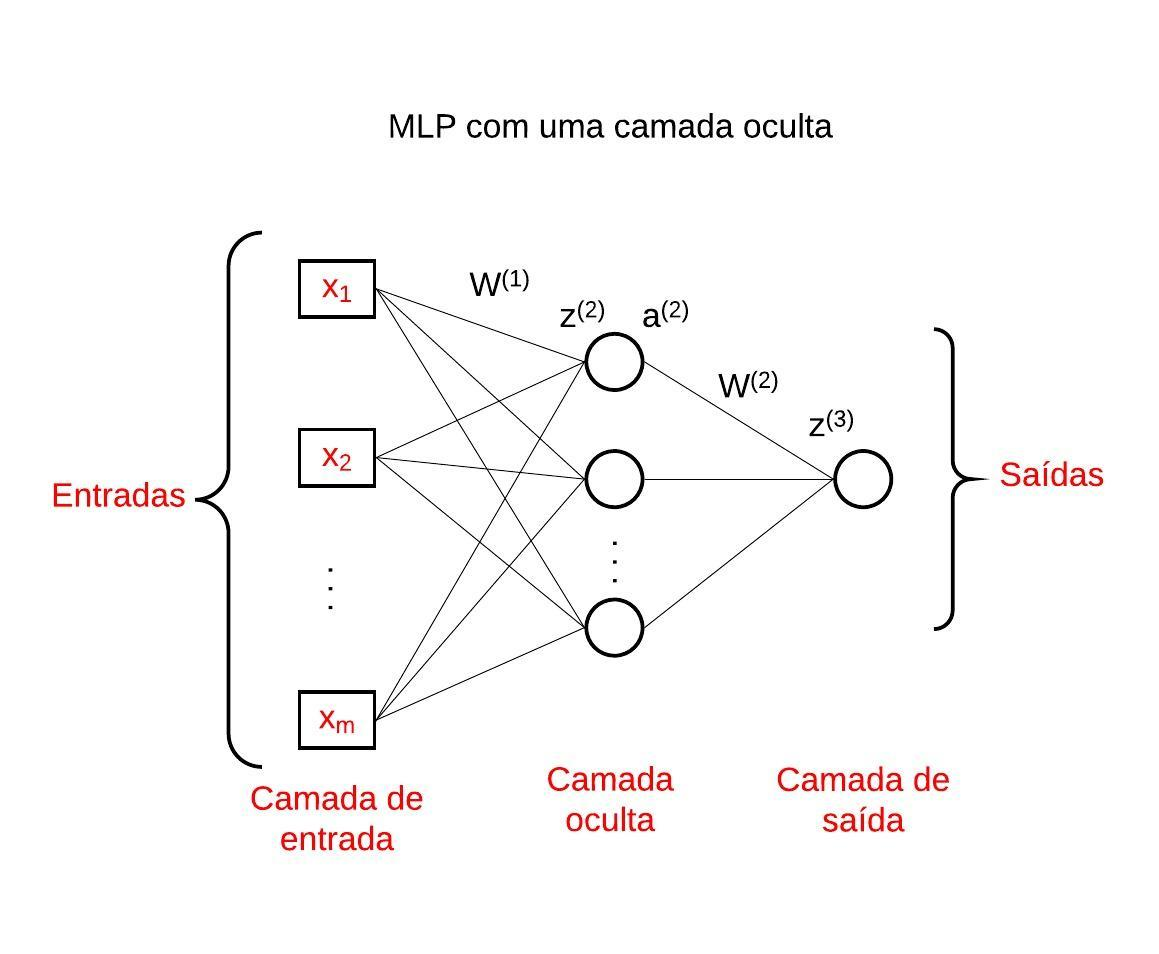
\includegraphics[width=350pt]{figuras/MLP_uma_camada.jpeg}
  \caption{MLP uma camada}
  \label{fig:MLP uma camada}
\end{figure}

A MLP \ref{fig:MLP uma camada} ilustrada acima tem uma camada de entrada, uma camada oculta e uma camada de saída. Abaixo será apresentado como ela irá predizer $\hat{y}$, e como este será aos poucos ser cada vez mais parecido com a resposta desejada $y$ depois de alguns ajustes de pesos sinápticos regrados pelas funções de custo de acordo com os vetores de pesos sinápticos $W^{(1)}$ e $W^{(2)}$ que minimizam a diferença entre $\hat{y}$ e $y$.

% Dado que $X_{r,c} = $ 
% $
%  \begin{pmatrix}
%   x_{1,1} & x_{1,2} & \cdots & x_{1,c} \\
%   x_{2,1} & x_{2,2} & \cdots & x_{2,c} \\
%   \vdots  & \vdots  & \ddots & \vdots  \\
%   x_{r,1} & x_{r,2} & \cdots & x_{r,c} 
%  \end{pmatrix}
% % \end{equation}
% $, que $y_{r} = $
% $
%  \begin{pmatrix}
%  y_{1} \\
%  y_{2} \\
%  \vdots  \\
%  y_{r}
%  \end{pmatrix}
% $
% e que $W_{r,c} = $
% $
% \begin{pmatrix}
%   w_{1,1} & w_{1,2} & \cdots & w_{1,c} \\
%   w_{2,1} & w_{2,2} & \cdots & w_{2,c} \\
%   \vdots  & \vdots  & \ddots & \vdots  \\
%   w_{r,1} & w_{r,2} & \cdots & w_{r,c}
% \end{pmatrix}
% $. 

Assumindo que $X = [x_1, x_2,...x_m]$ e que $W^{(1)}$ corresponde aos pesos sinápticos da primeira camada, tem-se que a ativação da segunda camada é dada por 

\begin{equation}
z^{(2)} = XW^{(1)}
\end{equation}

É necessário aplicar a função de ativação a cada valor de $z^{(2)}$, portanto tem-se que
\begin{equation}
a^{(2)} = f(z{(2)})
\end{equation}

Para finalizar a fase de propagação, é necessário propagar $a^{(2)}$ até o nó de saída da rede neural. Portanto, tem-se que a ativação da camanda de saída é dada por
\begin{equation}
z^{(3)} = a^{(2)}W^{(2)}
\end{equation}

Novamente é necessário aplicar a função de ativação a cada valor de $z^{(3)}$. Finalmente tem-se que $\hat{y}$ é dado por
\begin{equation}
\hat{y} = f(z^{(3)})
\end{equation}

Com isso, tem-se que o valor de saída da rede. Porém faz-se necessário determinar o quão certo ou errado a saída da rede $y$ é similar ao valor esperado $d$, ou seja, determina-se o custo.

\section{Função de custo}

O algoritmo de retropropagação procura encontrar pesos $w$ e biases $b$ de forma que a saída da rede neural $y$ se aproxime de todas as entradas $x$. Para quantificar o quão bem este objetivo está sendo alcançado, usa-se a função de custo, também conhecida por \textit{erro} ou \textit{função objetivo} representada pela equação abaixo:

\begin{equation}
\label{funcaodecusto}
C(w,b) = \sum_{i=1}^{r} \frac{1}{2}(y_i - \hat{y_i})^2    
\end{equation}

Neste caso, a função de custo quadrática, também conhecida como erro médio quadrático (MSE) é uma função positiva uma vez que todo termo somado é positivo. Além disso, o custo $C(w,b)$ se aproxima de zero quando $\hat{y}$ se aproxima de $y$. Portanto o algoritmo fez um bom trabalho se pôde encontrar pesos e biases de forma que $C(w,b) \approx 0$. O objetivo do algoritmo então é minimizar o custo em função dos pesos e biases.

% O custo é uma função de duas coisas: as entradas e os pesos. Como sabemos, não é possível alterar os dados de entrada, porém é possível alterar os pesos de forma que a função de custo seja minimizada, ou seja, procura-se uma combinação ótima dos valores de $W$ que resultem em um $J$ próximo ou igual a zero.

Quanto mais combinações tiverem que ser testadas, mais tempo computacional será necessário para encontrar a combinação ótima de $W$ que resulte num menor valor para a função de custo.

Usa-se a derivada parcial para determinar a taxa de variação de cada valor de $W^{(1)}$ em relação a função de custo. 

% O uso desta técnica para cada entrada da rede neural, indica em qual direção do plano formado pelas diferentes dimensões $w$ minimiza a função de custo em relação a $W^{(1)}$:

% \begin{equation}
% \dfrac{\partial J}{\partial W^{(1)}} = 
% \begin{pmatrix}
%   \dfrac{\partial J}{\partial w^{(1)}_{1,1}} & \dfrac{\partial J}{\partial w^{(1)}_{1,2}} & \cdots & \dfrac{\partial J}{\partial w^{(1)}_{1,c}} \\
%   \dfrac{\partial J}{\partial w^{(1)}_{2,1}} & \dfrac{\partial J}{\partial w^{(1)}_{2,2}} & \cdots & \dfrac{\partial J}{\partial w^{(1)}_{2,c}} \\
%   \vdots  & \vdots  & \ddots & \vdots  \\
%   \dfrac{\partial J}{\partial w^{(1)}_{r,1}} & \dfrac{\partial J}{\partial w^{(1)}_{r,2}} & \cdots & \dfrac{\partial J}{\partial w^{(1)}_{r,c}} \\
% \end{pmatrix}
% \end{equation}

% Já a função de custo de $W^{(2)}$ é dada por: 
% \begin{equation}
% \dfrac{\partial J}{\partial W^{(2)}} = 
% \begin{pmatrix}
%   \dfrac{\partial J}{\partial w^{(2)}_{1,1}} \\
%   \dfrac{\partial J}{\partial w^{(2)}_{2,1}} \\
%   \vdots \\
%   \dfrac{\partial J}{\partial w^{(2)}_{c,1}}
% \end{pmatrix}
% \end{equation}

% onde $c$ é o número de neurônios na camada oculta e $r$ é o número de entradas do conjunto de treinamento.

\begin{equation}
custo = \sum_{i=1}^{r} \frac{1}{2}(y_i - f(f(XW^{(1)})W^{(2)})^2    
\end{equation}

Deriva-se os dois lados da equação, assim tem-se:

\begin{equation}
    \frac{\partial J}{\partial W^{(2)}} = \partial \sum_{i=1}^{r} \frac{ \frac{1}{2}(y_i - \hat{y_i})^2}{\partial W^{(2)}}
\end{equation}

Como a soma das derivadas é o mesmo que a derivada das somas, é possível mover o somatório conforme segue:

\begin{equation}
    \frac{\partial J}{\partial W^{(2)}} = \sum_{i=1}^{r} \frac{\partial \frac{1}{2}(y_i - \hat{y_i})^2}{\partial W^{(2)}}
\end{equation}

Se considerado apenas o primeiro exemplar do conjunto de treinamento, ou seja, se consideramos apenas a primeira linha da matriz $X$, é possível omitir o somátório e adicionar cada um dos termos derivados depois:

\begin{equation}
    \frac{\partial J}{\partial W^{(2)}} = \frac{\partial \frac{1}{2}(y_i - \hat{y_i})^2}{\partial W^{(2)}}
\end{equation}

Por conta da regra da potenciação de derivada, tem-se:

\begin{equation}
    \frac{\partial J}{\partial W^{(2)}} = (y - \hat{y})
\end{equation}

Resta agora derivar a função $(y-\hat{y})$ em relação a $W^{(2)}$. 

O gráfico abaixo apresenta de maneira simplificada a rede neural com apenas um nó em cada camada.



% \begin{figure}[h]
%   \begin{tikzpicture}
%     %%Create a style for the arrows we are using
%     \tikzset{normal arrow/.style={draw,-triangle 45,very thick}}
%     %%Create the different coordinates to place the nodes
%     \path (0,0) coordinate (1) ++(0,-2) coordinate (2) ++(0,-2) coordinate (3);
%     \path (1) ++(-3,-.2) coordinate (x1);
%     \path (3) ++(-3, .2) coordinate (x2);
%     %%Use the calc library and partway modifiers to generate the second and third level points
%     \path ($(1)!.5!(2)!3 cm!90:(2)$) coordinate (4);
%     \path ($(2)!.5!(3)!3 cm!90:(3)$) coordinate (5);
%     \path ($(4)!.5!(5)!3 cm!90:(5)$) coordinate (6);
%     \path (6) ++(3,0) coordinate (7);
%     %%Place nodes at each point using the foreach construct
%     \foreach \i/\color in {1/Magenta!60,2/MidnightBlue!60,3/CadetBlue!80,4/CadetBlue!80,5/CadetBlue!80,6/CadetBlue!80}{
%       \node[draw,circle,shading=axis,top color=\color, bottom color=\color!black,shading angle=45] (n\i) at (\i) {$f_{\i}(e)$};
%     }
%     %%Place the remaining nodes separately
%     \node (nx1) at (x1) {$\mathbf{x_1}$};
%     \node (nx2) at (x2) {$\mathbf{x_2}$};
%     \node (ny)  at (7)  {$\mathbf{y}$};
%     %%Drawing the arrows
%     \path[normal arrow] (nx1) -- (n1);
%     \path[normal arrow] (nx1) -- (n3);
%     \path[normal arrow] (nx2) -- (n1);
%     \path[normal arrow] (nx2) -- (n3);
%     \path[normal arrow] (n1)  -- (n4);
%     \path[normal arrow] (n1)  -- (n5);
%     \path[normal arrow] (n2)  -- (n4);
%     \path[normal arrow] (n2)  -- (n5);
%     \path[normal arrow] (n3)  -- (n4);
%     \path[normal arrow] (n3)  -- (n5);
%     \path[normal arrow] (n4)  -- (n6);
%     \path[normal arrow] (n5)  -- (n6);
%     \path[normal arrow] (n6)  -- (ny);
%     %%Drawing the cyan arrows including the labels
%     \path[normal arrow,Cyan] (nx1) -- node[above=.5em,Cyan] {$\mathbf{w_{(x1)2}}$} (n2);
%     \path[normal arrow,Cyan] (nx2) -- node[below=.5em,Cyan] {$\mathbf{w_{(x2)2}}$} (n2);
%   \end{tikzpicture}
% \caption{Do not forget!
% Make it explicit enough that readers
% can figure out what you are doing.}
% \end{figure}

\begin{figure}[H]
    \centering
  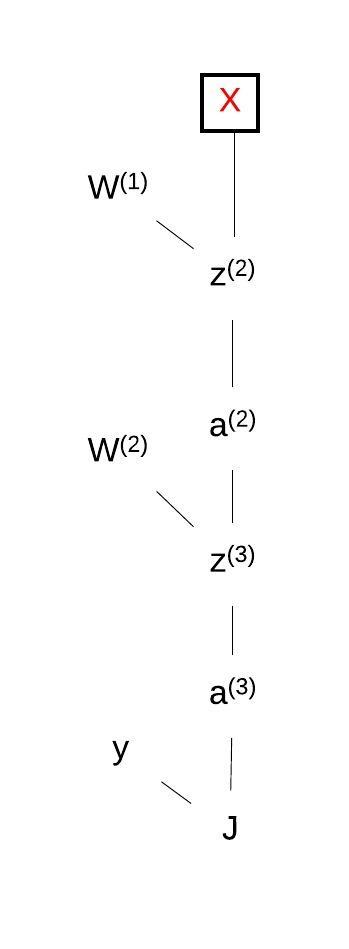
\includegraphics[width=100pt]{figuras/derivadas_parciais_um_no_por_camada.jpeg}
  \caption{Cálculo do custo}
  \label{fig:derivadas_parciais_um_no_por_camada}
\end{figure}

Assumindo que $a^{(3)}$ no gráfico acima representa $\hat{y}$ e aplicando a da regra da cadeia a fim determinar a \textit{sensibilidade} de $W^{(2)}$ em relação ao custo , tem-se:

\begin{equation}
    \frac{\partial J}{\partial W^{(2)}} = (y - \hat{y})(-\frac{\partial \hat{y}}{\partial z^{(3)}})
\end{equation}

Sabendo que $\hat{y}=f(z^{(3)})$, tem-se:
\begin{equation}
    \frac{\partial J}{\partial W^{(2)}} = -(y - \hat{y})\frac{\partial \hat{y}}{\partial z^{(3)}}\frac{\partial z^{(3)}}{\partial W^{(2)}}
\end{equation}

$\frac{\partial \hat{y}}{\partial z^{(3)}}$ representa aqui a derivada da função de ativação, portanto será representada por $f'(z^{(3)})$ como mostrado abaixo:
\begin{equation}
    \frac{\partial J}{\partial W^{(2)}} = -(y - \hat{y}) f'(z^{(3)}) \frac{\partial z^{(3)}}{\partial W^{(2)}}
\end{equation}

Sabendo que $z^{(3)}=a^{(2)}W^{(2)}$, temos que $a^{(2)}$, é a taxa de variação de $z^{(3)}$ em relação a $W^{(3)}$.

$-(y-\hat{y})$ representa a seguinte matriz:

\begin{equation*}
\begin{pmatrix}
  -y_1 - \hat{y}_1\\
  -y_2 - \hat{y}_2\\
  \vdots \\
  -y_r - \hat{y}_r
\end{pmatrix}
\end{equation*}

Já $f'(z^{(3)})$ representa a seguinte matriz:

\begin{equation*}
\begin{pmatrix}
  f'(z^{(3)}_1)\\
  f'(z^{(3)}_2)\\
  \vdots \\
  f'(z^{(3)}_r)
\end{pmatrix}
\end{equation*}

A multiplicação destas matriz resulta noutra matriz $\delta^{(3)}$ conforme segue:

\begin{equation*}
\begin{pmatrix}
  \delta_1^{(3)}\\
  \delta_2^{(3)}\\
  \vdots \\
  \delta_r^{(3)}
\end{pmatrix}
\end{equation*}

A equação $ z^{(3)} = a^{(2)} W^{(2)} $ representa a ativação da segunda camada que é dada por $(a^{(2)})^T$, portanto tem-se que que o custo da terceira camada é dado por:

\begin{equation}
    \frac{\partial J}{\partial W^{(2)}} = (a^{(2)})^T \delta^{(3)}
\end{equation}

O mesmo processo é feito para se determinar o custo da primeira camada, portanto tem-se:

\begin{equation}
    \frac{\partial J}{\partial W^{(1)}} = \delta^{(3)} \frac{\partial z^{(3)}}{\partial a^{(2)}} \frac{\partial a^{(2)}}{\partial W^{(1)}}
\end{equation}

\begin{equation}
    \frac{\partial J}{\partial W^{(1)}} = \delta^{(3)} \frac{\partial z^{(3)}}{\partial a^{(2)}} \frac{\partial a^{(2)}}{\partial z^{(2)}} \frac{\partial z^{(2)}}{\partial W^{(1)}}
\end{equation}

Fazendo as devidas substituições:
\begin{equation}
    \frac{\partial J}{\partial W^{(1)}} = \delta^{(3)} (W^{(2)})^T f'(z^{(2)}) \frac{\partial z^{(2)}}{\partial W^{(1)}}
\end{equation}

Finalmente, usando a transposta da matriz X, tem-se a seguinte equação que representa o custo da primeira camada:
\begin{equation}
    \frac{\partial J}{\partial W^{(1)}} = X^T \delta^{(3)} (W^{(2)})^T f'(z^{(2)})
\end{equation}

Resumindo, tem-se que a correção $\Delta w_{ij}(n)$ aplicada ao peso da conexão sináptica do neurônio $i$ da camada $j$ é definida por:

\begin{equation*}
    \begin{pmatrix} 
    \text{Correção do peso} \\
    \Delta w_{ij}(n)
    \end{pmatrix}
    =
    \begin{pmatrix} 
    \text{taxa de aprendizado} \\ 
    \eta
    \end{pmatrix}
    \times
    \begin{pmatrix} 
    \text{gradiente local} \\ 
    \delta_j(n)
    \end{pmatrix}
    \times
    \begin{pmatrix} 
    \text{entrada do neurônio $j$} \\ 
    $y$_i(n)
    \end{pmatrix}
\end{equation*}

O grandiente local $\delta_j(n)$ depende se o neurônio $j$ é oculto ou de saída:
\begin{enumerate}
    \item Se o neurônio $j$ for de saída, $\delta_j(n)$ é igual ao produto da derivada $\phi_j'(v_j(n))$ pelo erro $e_j(n)$ no neurônio $j$;
    \begin{equation*}
        \delta_j(n) = e_j(n)\phi'_j(v_j(n))
    \end{equation*}
    \item Se o neurônio $j$ for oculto, $\delta_j(n)$ é igual ao produto da derivada $\phi_j'(v_j(n))$ pelas somas ponderadas de $\delta$ calculado para o neurônio na próxima camada que está conectado ao neurorio $j$.
    \begin{equation*}
        \delta_j(n) = \phi'_j(v_j(n)) \sum_k \delta_k(n)w_{kj}(n)
    \end{equation*}
\end{enumerate}

\subsection{Funções de ativação}

Nesta seção será apresentado porque é conveniente usar funções do tipo sigmoid em redes de múltiplas camadas.
O cálculo de $\delta$ para cada neurônio $j$ requer a derivada da função $\phi$ associada aquele neurônio. O único requisito para que a derivada desta função exista, é que a função seja contínua.
Um exemplo de função contínua não linear é a sigmoid (nome proveniente de sigma que é a letra s do alfabeto grego por conta do formato apresentado quando esta função é plotada.
Duas formas de sigmoid são apresentadas abaixo:

\begin{enumerate}
    \item Função logística:
    \begin{figure}[H]
    \centering
    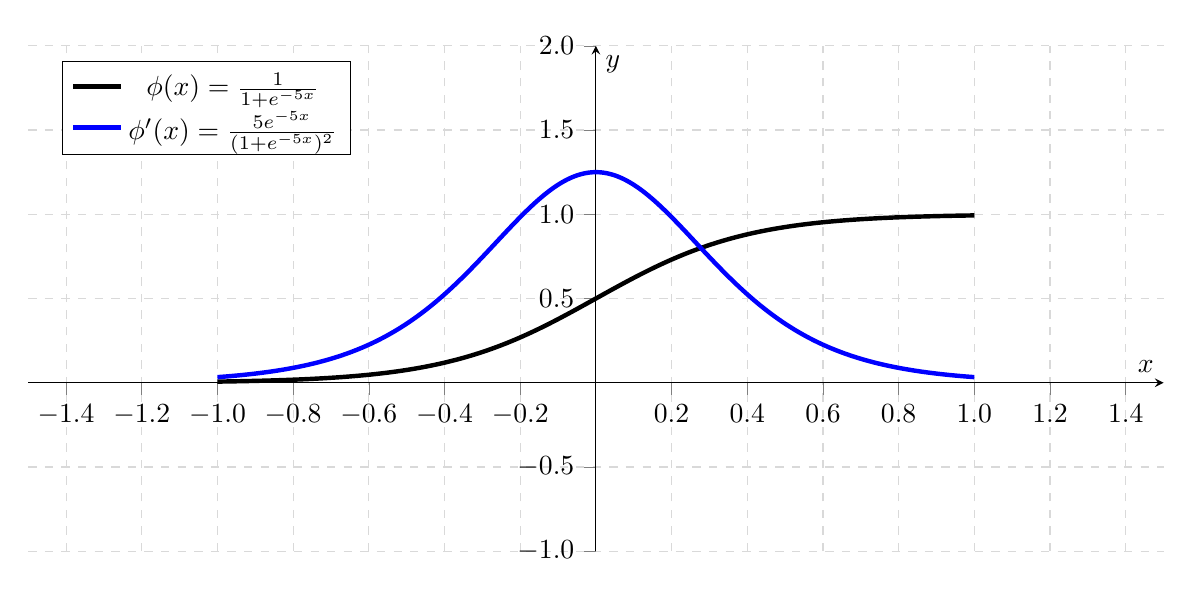
\begin{tikzpicture}
    \begin{axis}[
    	legend pos=north west,
        axis x line=middle,
        axis y line=middle,
        x tick label style={/pgf/number format/fixed,
                            /pgf/number format/fixed zerofill,
                            /pgf/number format/precision=1},
        y tick label style={/pgf/number format/fixed,
                            /pgf/number format/fixed zerofill,
                            /pgf/number format/precision=1},
        grid = major,
        width=16cm,
        height=8cm,
        grid style={dashed, gray!30},
        xmin=-1.5, xmax= 1.5,
        ymin= -1, ymax= 2,
        domain=-1:1,
        %axis background/.style={fill=white},
        xlabel=$x$,
        ylabel=$y$,
        tick align=outside,
        enlargelimits=false]
      % plot the stirling-formulae
      \addplot[ultra thick,samples=500] {1/(1+exp(-5*x))};
      \addplot[blue, ultra thick, samples=500]{(5*exp(-5*x))/((exp(-5*x)+1)*(exp(-5*x)+1))};
      \addlegendentry{$\phi(x)=\frac{1}{1+e^{-5x}}$}
      \addlegendentry{$\phi'(x)=\frac{5e^{-5x}}{(1+e^{-5x})^2}$}
    \end{axis}
    \end{tikzpicture}
    \caption{Gráfico da função logística e sua derivada}
    \end{figure}
    \begin{equation}
        \phi(x) = \frac{1}{1+e^{-\alpha x}}, \: com \: \alpha > 0
    \end{equation}
    Diferenciando esta função em relação a $x$, tem-se:
    \begin{equation}
        \frac{\partial \phi(x)}{\partial x} = \frac{\partial (1+e^{-\alpha x})^{-1}}{\partial x}
    \end{equation}
    Resolvendo a equação de acordo com a regra da potência de derivada, tem-se:
    \begin{equation}
        \frac{\partial \phi(x)}{\partial x} = (1+e^{-\alpha x})^{-2} (e^{-\alpha x}) \alpha
    \end{equation}
    Reescrevendo a equação acima, tem-se:
    \begin{equation}
        \frac{\partial \phi(x)}{\partial x} = \left(\frac{1}{1+e^{-\alpha x}}\right) \left(\frac{e^{-\alpha x}}{1+e^{-\alpha x}} \right) \alpha
    \end{equation}
    Adicionando e subtraindo 1 do numerador da segunda parcela da equação, tem-se:
    \begin{equation}
        \frac{\partial \phi(x)}{\partial x} = \left(\frac{1}{1+e^{-\alpha x}}\right) \left(\frac{\textbf{1}+e^{-\alpha x} - \textbf{1}}{1+e^{-\alpha x}}\right) \alpha
    \end{equation}
    Expandindo a equação acima, tem-se:
    \begin{equation}
        \frac{\partial \phi(x)}{\partial x} = \left(\frac{1}{1+e^{-\alpha x}}\right) \left(\frac{1+e^{-\alpha x}}{1+e^{-\alpha x}} - \frac{1}{1+e^{-\alpha x}}\right) \alpha
    \end{equation}
    Lembrando que $\frac{1}{1+e^{-\alpha x}} = \phi(x)$ e fazendo as devidas substituições, tem-se:
    \begin{equation}
        \frac{\partial \phi(x)}{\partial x} = \phi(x) (1- \phi(x)) \alpha
    \end{equation}
    Essa simplificação permite que o cálculo do gradiente local para qualquer neurônio $j$ seja dado por:
        \begin{itemize}
        \item Para neurônios da camada de saída:
        \begin{equation}
            \begin{split}
            \delta_j(n) = e_j(n)\phi'(v_j(n)) \\
            \delta_j(n) = \alpha[y_j(n) - \hat{y_j}(n)]\hat{y_j}(n)[1 - \hat{y_j}(n)]    
            \end{split}
        \end{equation}
        \item Para neurônios da camada oculta:
        \begin{equation}
            \begin{split}
            \delta_j(n) = \phi'(v_j(n)) \sum_k \delta_k(n)w_{kj}(n) \\
            \delta_j(n) = \alpha y_j(n)[1 - y_j(n)]\sum_k \delta_k(n)w_{kj}(n)
            \end{split}
        \end{equation}
    \end{itemize}
Percebe-se que a função $\phi'(x)=x*(1-x)$, em azul, tem máximo em 0.5 e mínimos em 0 e 1.0. Considerando que o ajuste num peso sináptico é proporcional a derivada $\phi_j(v_j(n))$, os pesos que têm mais influência no ajuste, são aqueles que têm ativação nos seus intervalos intermediários. De acordo com David Rumelhart (\citeyear{rumelhart1986parallel}), é essa característica do algoritmo de retro-propagação que contribui para sua estabilidade como algoritmo de aprendizado.
\item Função tangente hiperbólica
    \begin{figure}[H]
    \centering
    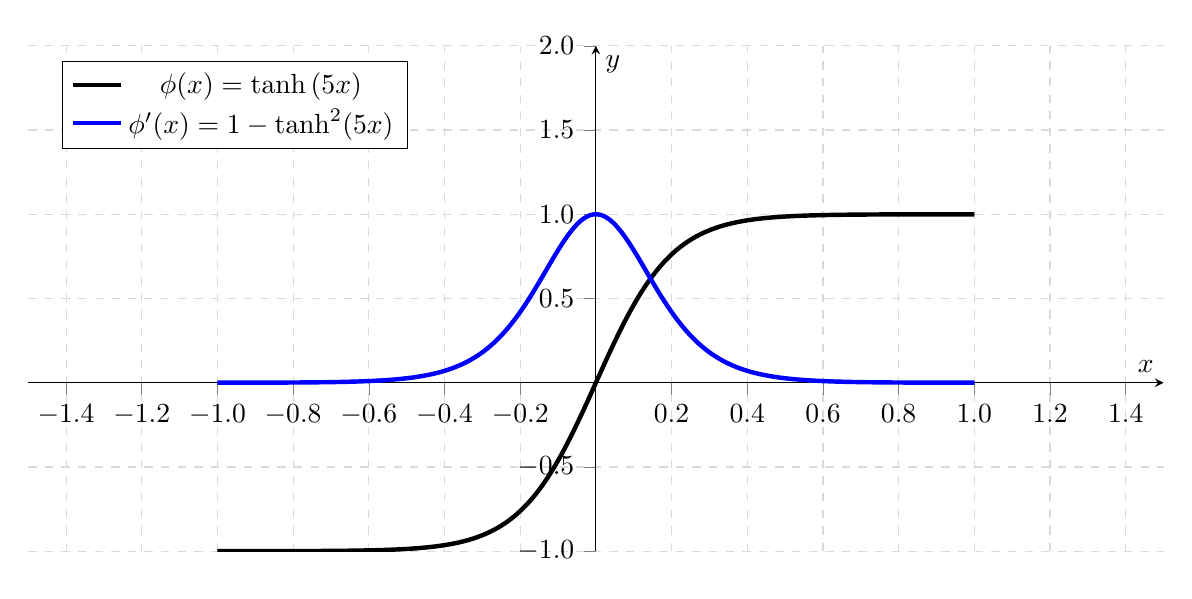
\begin{tikzpicture}
    \begin{axis}[
    	legend pos=north west,
        axis x line=middle,
        axis y line=middle,
        x tick label style={/pgf/number format/fixed,
                            /pgf/number format/fixed zerofill,
                            /pgf/number format/precision=1},
        y tick label style={/pgf/number format/fixed,
                            /pgf/number format/fixed zerofill,
                            /pgf/number format/precision=1},
        grid = major,
        width=16cm,
        height=8cm,
        grid style={dashed, gray!30},
        xmin=-1.5, xmax= 1.5,
        ymin= -1, ymax= 2,
        domain=-1:1,
        %axis background/.style={fill=white},
        xlabel=$x$,
        ylabel=$y$,
        tick align=outside,
        enlargelimits=false]
      % plot the stirling-formulae
    \addplot[ultra thick,samples=500] {tanh(5* \x)};
      \addplot[blue, ultra thick, samples=500]{1-((tanh(5* \x) * (tanh(5* \x)))};
    %   \addplot[yellow, ultra thick, samples=500]{5[}
      \addlegendentry{$\phi(x)=\tanh{(5x)}$}
      \addlegendentry{$\phi'(x)= 1 - \tanh^2(5x)$}
    \end{axis}
    \end{tikzpicture}
    \caption{Gráfico da função tangente hiperbólica e sua derivada}
    \end{figure}
Outra forma de função sigmoid é a tangente hiperbólica, cuja equação mais geral é dada por:

\begin{equation}
    \phi(x)=a*tanh(b*x)
\end{equation}

onde a e b são constantes positivas. Na verdade, esta função é função logística re-escalada e tendenciosa.
Sua derivada em relação a $x$ é dada por:
\begin{equation}
    \begin{split}
    \phi'(x)=ab(sech^2(bx) \\
    \phi'(x)=ab(1-tanh^2(bx) \\
    \phi'(x)=\frac{b}{a}[a-x][a+x]
    \end{split}
\end{equation}
\begin{itemize}
    \item Para um neurônio $j$ na camada de saída, tem-se:
        \begin{equation}
            \begin{split}
                \delta_j(n)=e_j(n)\phi'(v_j(n)) \\
                \delta_j(n)=\frac{b}{a}[y_j(n)-\hat{y}_(n)][a-\hat{y}_(n)][a+\hat{y}_(n)]
            \end{split}
        \end{equation}
    \item Para um neurônio $j$ na camada oculta, tem-se:
    \begin{equation}
        \begin{split}
        \delta_j(n) = \phi'(v_j(n)) \sum_k \delta_k(n)w_{kj}(n) \\
        \delta_j(n) = \frac{b}{a}[a-y_j(n)][a+y_j(n)] \sum_k \delta_k(n)w_{kj}(n)
        \end{split}
    \end{equation}
\end{itemize}
\end{enumerate}

\subsection{Taxa de aprendizado e constante momentum}

O perceptron de múltiplas camadas aprende ao passo que ajusta os pesos de acordo com a função de custo. A velocidade com que se dá o aprendizado depende de algums fatores como valor inicial de cada peso, escala de cada atributo de entrada, taxa de aprendizado e constante momentum. Nesta seção será explicado como a taxa de aprendizado e o valor do momemtum afetam a velocidade do aprendizado da rede e o que deve ser considerado para determinar seus valores.

O algoritmo de retro propagação procura encontrar os valores dos pesos sinápticos que minimizam a função de custo. Para isso, usa-se o gradiente descendente que como foi explicado em seções acima, é dado pela derivada do custo em relação aos pesos. Segue uma forma lúdica de como o algoritmo faz isso: Imagine que você está numa montanha com muita névoa e que seu objetivo é descer antes do pôr do sol.
Você decide olhar em volta e ir para o ponto mais baixo ao seu redor, porém há tanta névoa que você não enxerga. Por sorte, você tem um aparelho  que mensura a inclinação. Você aponta o aparelho para chão num ponto próximo a você e compara com as medições a sua volta.
Você anda para o ponto mais baixo. Se você repetir esse processo, eventualmente chegará na base da montanha. Mas tem um problema, a medição com o aparelho leva um tempo. Então seu objetivo é usar menos o aparelho para que alcance a base da montanha antes do pôr do sol. 
Você representa o algoritmo. 

A montanha representa a função de custo. A base da montanha representa o mínimo global. A inclinação medida pelo aparelho representa a inclinação da superfície de erro naquele ponto. O aparelho usado para medir a inclinação é a derivada do função de erro quadrado naquele ponto. A direção escolhida para descer está alinhada com o gradiente da superfície de erro naquele ponto. O tempo que leva para descer até o ponto mais baixo local é a taxa de aprendizado.
Quanto menor o valor da taxa de aprendizado, mais suave é a trajetória na superfície de erro. Por outro lado, um valor alto para a taxa de aprendizado, por mais que acelere o aprendizado, pode resultar em uma trajetória que oscila e que demore para convergir até encontrar o mínimo.

Um método simples de modificar a taxa de aprendizado de forma dinâmica a fim de evitar o perigo da instabilidade, é incluir um termo momentum na regra de ajuste de peso sináptico conforme segue:

\begin{equation}
\Delta w_{ij}(n) = \alpha \Delta w_{ij}(n-1) + \eta \delta_j(n)y_i(n)
\end{equation}

\begin{figure}[H]
  \centering
  \begin{subfigure}[b]{0.4\linewidth}
    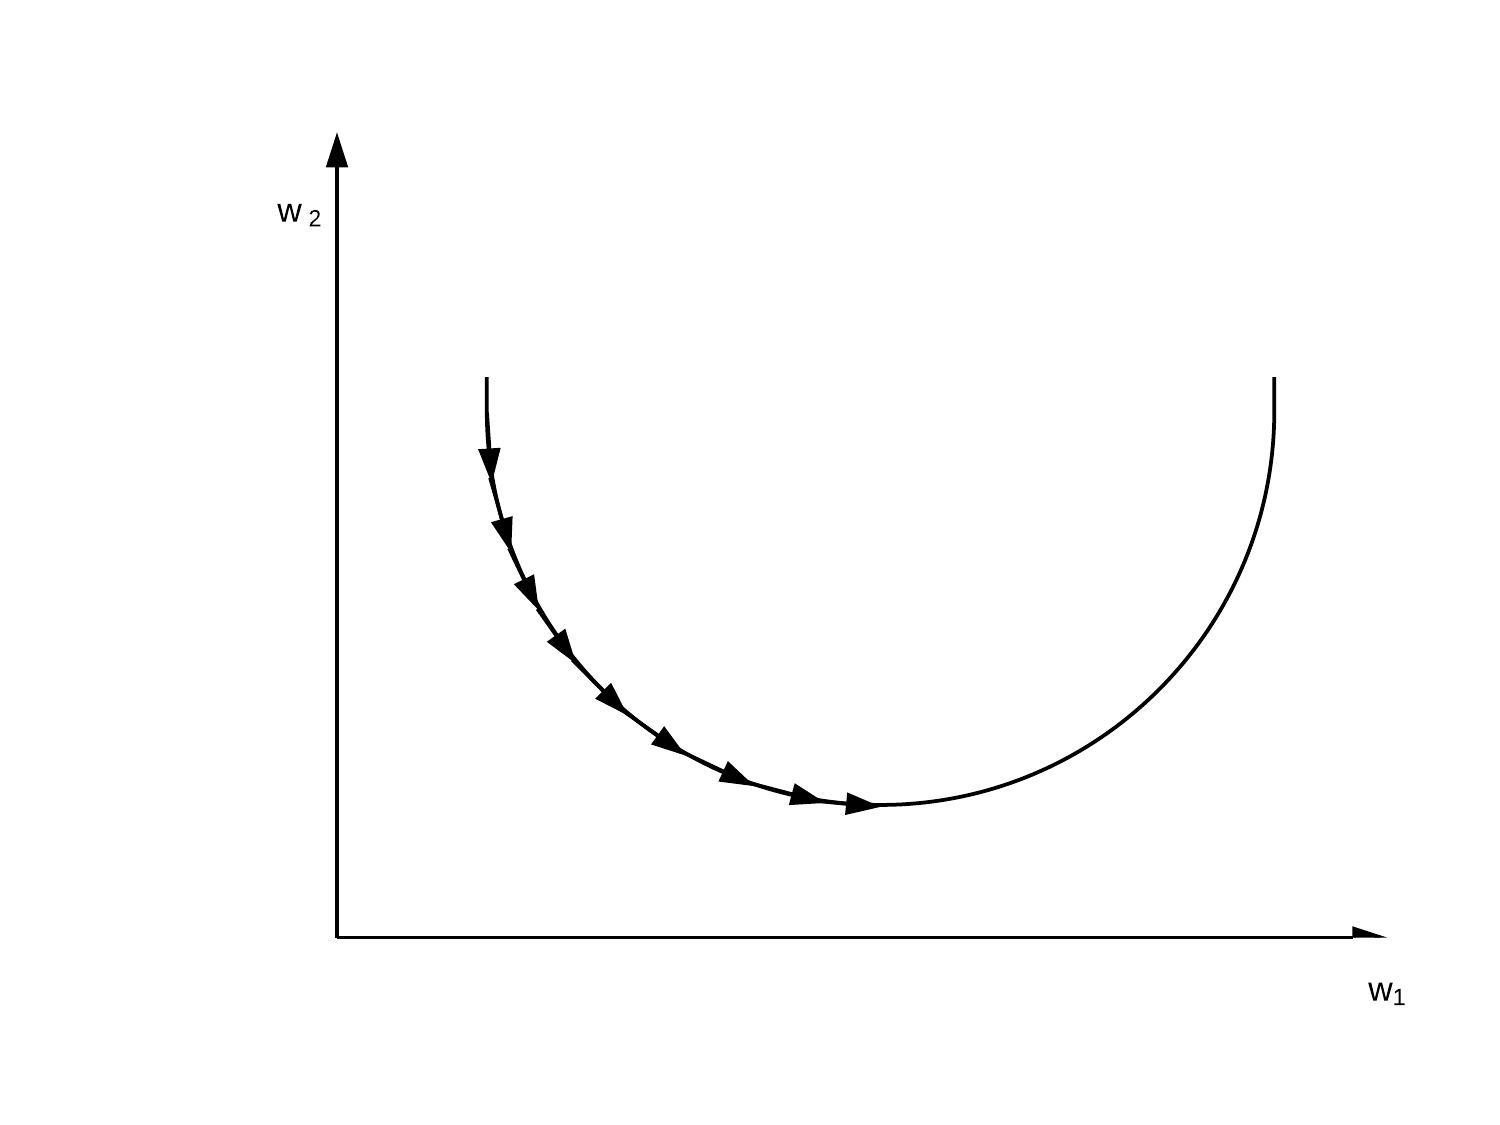
\includegraphics[width=\linewidth]{figuras/Sem_momentum.jpeg}
    \caption{Sem momentum}
  \end{subfigure}
  \begin{subfigure}[b]{0.4\linewidth}
    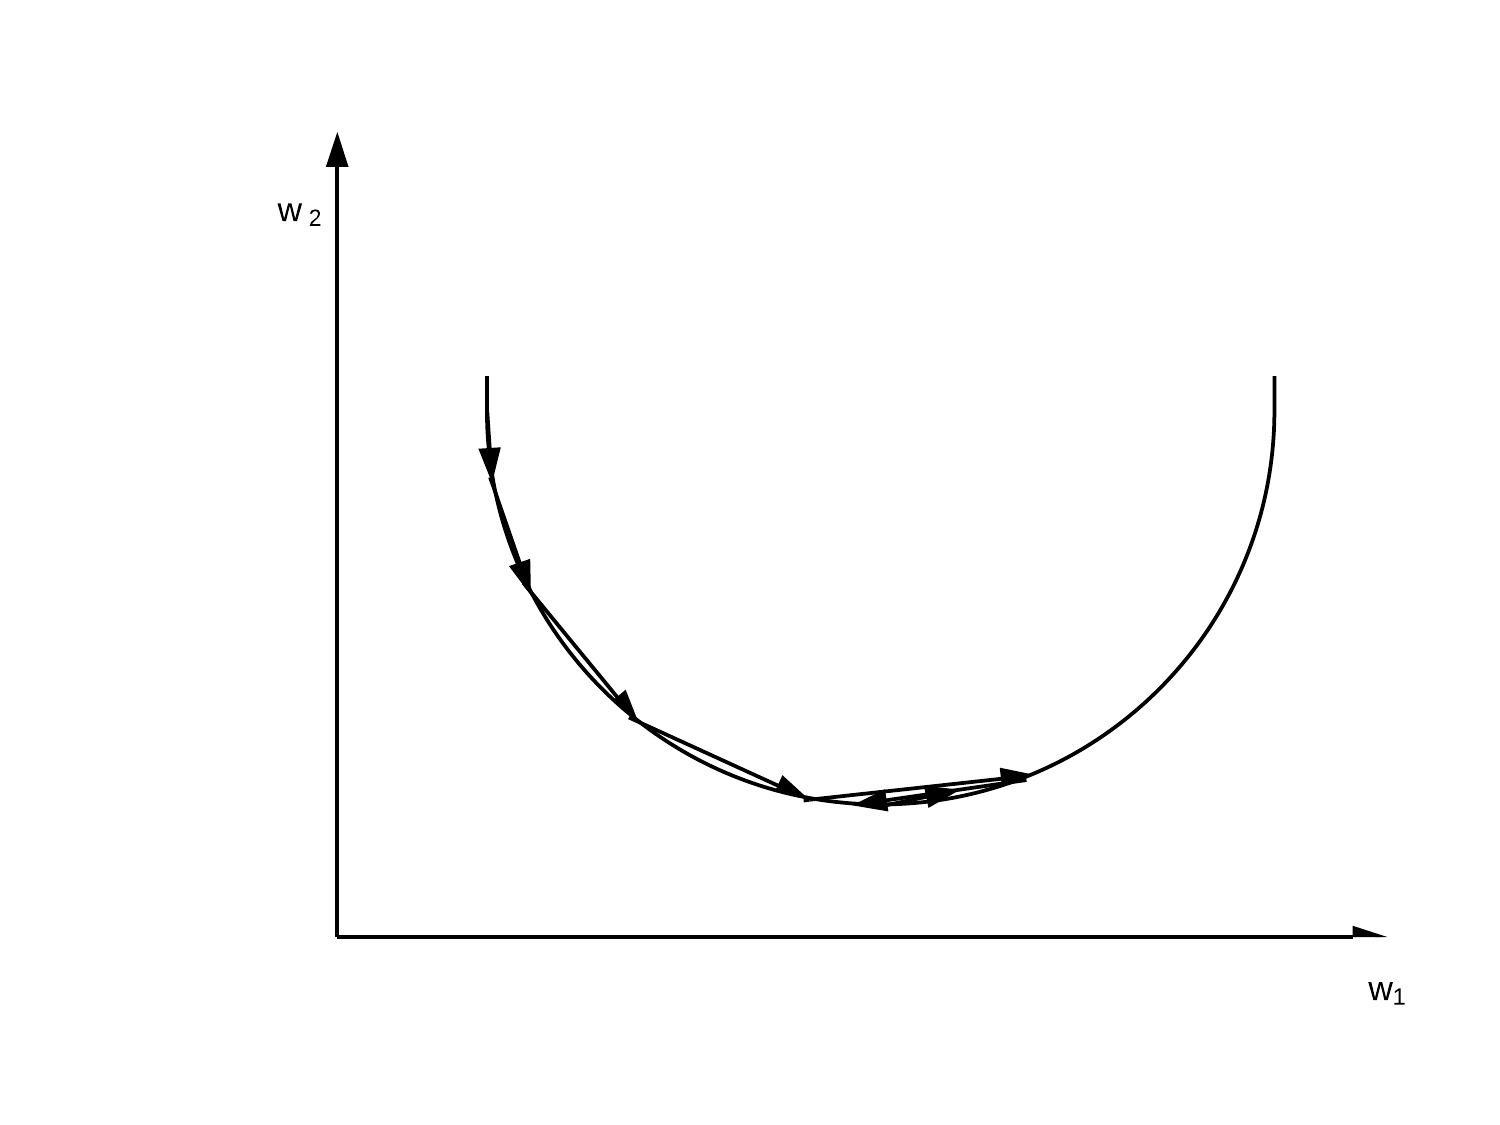
\includegraphics[width=\linewidth]{figuras/Com_momentum.jpeg}
    \caption{Com momemtum}
  \end{subfigure}
  \caption{Comparação de uso de momentum}
  \label{fig:coffee}
\end{figure}

Sabe-se que $\delta_j(n)y_i(n)$ é dado por $\frac{-\partial e(n)}{\partial w_{ij}(n)}$. Quando esta derivada em particular tem o mesmo sinal em várias iterações sucessivas, o ajuste de $\Delta w_{ij}(n)$ cresce, portanto a inclusão do momentum tende a acelerar o aprendizado.

Quando a derivada $\frac{\delta e(n)}{\delta w_{ij}(n)}$ tem o sinal oposto em iterações sucessivas, o ajuste diminui. Portanto a inclusão do momentum tende a estabilizar o efeito de oscilação durante o aprendizado.

\section{Validação Cruzada}

\begin{figure}[H]
  \centering
  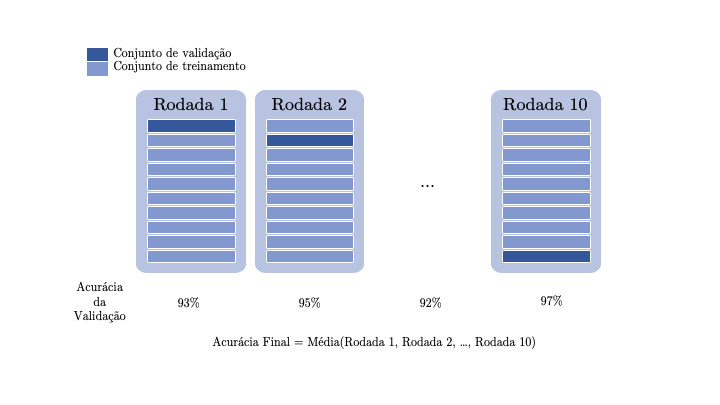
\includegraphics[width=450pt]{figuras/validacao_cruzada.png}
  \caption{Ilustração de multi-pastas no método de validação cruzada. Para uma rodada, o subconjunto dos dados destacados azul escuro é usado para validar o modelo treinado com o restante dos dados.}
  \label{fig:validacao_cruzada}
\end{figure}

Em essência o algoritmo de retropropagação codifica um mapeamento entrada-saída em uma rede neural perceptron de múltiplas camadas. Espera-se que a rede seja tão bem treinada com os dados passados, que consiga generalizar o futuro. Nessa perspectiva, o processo de aprendizado envolve encontrar o conjunto de parâmetros ou estrutura de acordo com um certo critério.

Uma ferramenta/técnica estatística conhecida como validação cruzada \cite{stone1974cross} permite testar o modelo com um conjunto de dados diferente do qual foi usado para parametrizar a rede neural.

Para isso, ordena-se o conjunto de dados de forma aleatória que é então dividido em amostra de treinamento e conjunto de teste. A amostra de treinamento é então particionada em dois conjuntos disjuntos:

\begin{itemize}
    \item um subconjunto de estimação usado para parametrizar o modelo
    \item um subconjunto de validação usado para testar/validar o modelo
\end{itemize}

Testar o modelo com o sub-conjunto de teste previne que o modelo seja incapaz de generalizar.
O problema então é como determinar o parâmetro $r$ que determine a divisão da amostra de treinamento entre o subconjunto de estimação e o subconjunto de validação. Em um estudo \cite{kearns1996bound} foi identificado que o valor $0.1$ funciona de maneira quase ótima para uma grande variedade de cenários. Ou seja, $90\%$ do conjunto de dados é destinado ao subconjunto de estimação e o restante $10\%$ é destinado ao subconjunto de validação.